\documentclass[tikz,border=8pt]{standalone}
\usepackage{amsmath}
\usetikzlibrary{arrows.meta,calc,positioning}
\definecolor{ink}{HTML}{21352F}
\definecolor{teal}{HTML}{087F7B}
\definecolor{blue}{HTML}{4B77A8}
\definecolor{gold}{HTML}{C58B2A}
\definecolor{rose}{HTML}{B65A62}
\begin{document}
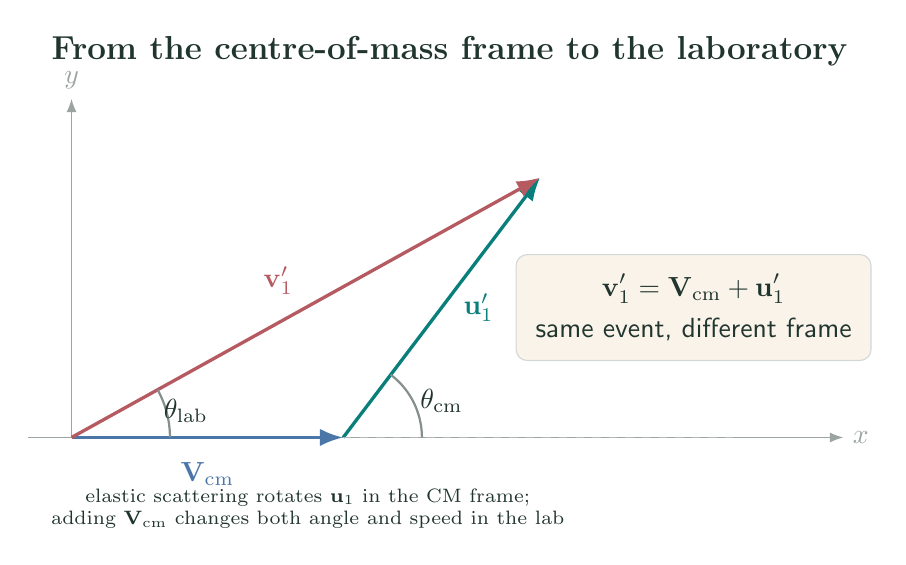
\begin{tikzpicture}[font=\sffamily,text=ink,>=Latex]
  \pgfmathsetmacro{\cmangle}{atan(3.30/2.50)}
  \pgfmathsetmacro{\labangle}{atan(3.30/5.95)}
  \node[font=\bfseries\large] at (0,3.65)
    {From the centre-of-mass frame to the laboratory};

  \coordinate (O) at (-4.8,-1.25);
  \coordinate (C) at (-1.35,-1.25);
  \coordinate (F) at (1.15,2.05);

  \draw[->,ink!45] (-5.35,-1.25)--(5.0,-1.25)
    node[right] {$x$};
  \draw[->,ink!45] (O)--(-4.8,3.05) node[above] {$y$};

  \draw[blue,very thick,->] (O)--(C)
    node[midway,below=5pt] {$\mathbf V_{\rm cm}$};
  \draw[teal,very thick,->] (C)--(F)
    node[midway,right=4pt] {$\mathbf u_1'$};
  \draw[rose,very thick,->] (O)--(F)
    node[midway,above left=1pt] {$\mathbf v_1'$};
  \draw[ink!35,dashed] (C)--(3.7,-1.25);

  \draw[ink!55,thick] ($(C)+(1.0,0)$)
    arc[start angle=0,end angle=\cmangle,radius=1.0];
  \node at (-.1,-.78) {$\theta_{\rm cm}$};
  \draw[ink!55,thick] ($(O)+(1.25,0)$)
    arc[start angle=0,end angle=\labangle,radius=1.25];
  \node at (-3.35,-.91) {$\theta_{\rm lab}$};

  \node[draw=ink!20,fill=gold!10,rounded corners=4pt,
        align=center,inner sep=7pt] at (3.1,.4)
    {$\displaystyle\mathbf v_1'
      =\mathbf V_{\rm cm}+\mathbf u_1'$\\[3pt]
     same event, different frame};

  \node[font=\scriptsize,align=center] at (-1.8,-2.15)
    {elastic scattering rotates $\mathbf u_1$ in the CM frame;\\
     adding $\mathbf V_{\rm cm}$ changes both angle and speed in the lab};
\end{tikzpicture}
\end{document}
